\section{Versuchsaufbau und Durchführung}
\label{sec:Durchführung}

Für diesen Versuch wird ein gedämpfter Schwingkreis benutzt.
Der Schwingkreis ist in Form der \textit{Drillachse}, welche in Abbildung \ref{fig:drillachse} zu erkennen ist, vorliegend.
Dabei handelt es sich um eine Apperatur, bei der ein beliebiger Körper eingespannt werden kann.
Diese ist mit der Winkelrichtgröße $D$ verknüpft.

\subsection{Bestimmung der Winkelrichtgröße $\pmb{D}$ und des Eigenträgheitsmomentes $\pmb{i_{D}}$} \label{subsec:Winkelrichtgröße}

\begin{figure}[H]
    \centering
    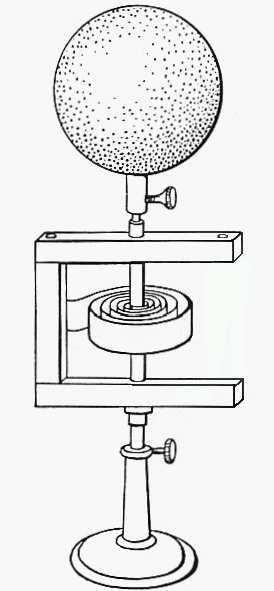
\includegraphics{pictures/Drillachse.png}
    \caption{Aufbau der Drillachse \cite{v101}.}
    \label{fig:drillachse}
\end{figure}

Zunächst wird die charakteristische Winkelrichtgröße $D$ der Drillachse gemessen.
Dazu wird als Erstes ein Stab eingespannt.
Um die Berechnung zu vereinfachen, wird dieser als masselos angenommen.
Es wird nun wie in Kapitel \ref{sec:statmethode} vorgegangen.
Zunächst wird mithilfe der \textbf{statischen Methode} die Kraft $F$ gemessen, die benötigt wird,
den Stab um den Winkel $\varphi$ auszulenken.
Es wird auch der Radius $r$ notiert, an der das Newtonmeter angebracht wird.
Hier sei erneut angemerkt, dass das Newtonmeter möglichst senkrecht an den Stab angebracht wird.
Deshalb wird der Winkel als $\vartheta = \frac{\pi}{2}$ angenommen.
Die Messung wird in 10° Schritten von $\varphi = 20°$ auf $\varphi = 120°$ durchgeführt. \\

Nun wird zur \textbf{dynamischen Methode} übergegangen, um das Eigenträgheitsmoment $I_{D}$ zu bestimmen.
Der Ablauf dieser Methode wurde in Kapitel \ref{sec:dynmethode} ausgeführt.
Dafür werden auf dem eingespannten Stab zwei Gewichte symmetrisch zur Mitte mit Radius $r$ angebracht.
Danach wird dieser Aufbau um den Winkel $\varphi = \frac{\pi}{2}$ ausgelenkt und losgelassen.
Dieser schwingt nun um die Ruhelage mit einer Schwingungszeit $T$.
Es werden Radius $r$ und Schwingungszeit $T$ notiert.
Die Messung wird ebenfalls 10 Mal für verschieden Radien durchgeführt.


\subsection{Bestimmung der Trägheitsmomente einer Kugel und eines Zylinders}
Nun werden jeweils eine Kugel und ein Zylinder vermessen und eingespannt.
Um das Trägheitsmoment dieser Körper zu bestimmen, wird analog zu Kapitel \ref{subsec:Winkelrichtgröße} vorgegangen.
Dieser Prozess wird für beide Körper 10-fach durchgeführt.

\subsection{Trägheitsmoment einer Holzpuppe}
Hierfür wird eine Holzpuppe eingespannt und es soll für zwei verschiedene Posen das Trägheitsmoment bestimmt werden.
Die Puppe wird bei der einer Pose so ausgerichtet, dass die Arme abstehen.
Bei der anderen Pose wird sie so ausgericht, dass die Beine in einem 90° Winkel zum Torso stehen.
Auch hier wird analog zu Kapitel \ref{subsec:Winkelrichtgröße} vorgegangen.
Allerdings müssen dabei die Maße des Körpers aufwendiger aufgenommen werden, da es sich nun nicht mehr um ein symmetrisches Objekt handelt.
Es werden also verschiedene Durchmesser an den Gliedmaßen gemessen und es wird zur Approximation ein Mittelwert gebildet.